\documentclass[11pt,a4paper,openany,oneside,parskip=half*]{article}

\usepackage[utf8]{inputenc}
\usepackage{tocloft}
\usepackage{nomencl}
\usepackage{pdfpages}
\usepackage{scrextend}
\usepackage{bm}
\usepackage{cite}
\usepackage{amsmath}
\usepackage{graphicx}
\usepackage[justification=justified]{caption}
\usepackage{float}
\usepackage{multicol}
\usepackage{float}
\usepackage[section]{placeins}
\usepackage[english]{babel} 
\usepackage{geometry} %Gr�ߟe des Bodys innerhalb der Seite 
\usepackage[utf8]{inputenc} 
\usepackage{ifthen}
\usepackage{caption}

%bindet die benutzten Packages ein

\linespread{1.25}

\captionsetup{width=0.485\linewidth}

\RequirePackage{ifthen}
\renewcommand{\nomgroup}[1]{%
  \ifthenelse{\equal{#1}{R}}{\item[\textbf{Roman Symbols}]}{%
    \ifthenelse{\equal{#1}{G}}{\item[\textbf{Greek Symbols}]}{%
      \ifthenelse{\equal{#1}{O}}{\item[\textbf{Operators}]}{%
	\ifthenelse{\equal{#1}{A}}{\item[\textbf{Acronyms}]}{}}}}}%
	
\renewcommand*\vec[1]{\boldsymbol{#1}}
\renewcommand*\matrix[1]{\boldsymbol{#1}}

\captionsetup[figure]{font=footnotesize}

\cftsetindents{section}{0em}{2.65em}   
\cftsetindents{subsection}{1.5em}{3em}   
\cftsetindents{subsubsection}{2.5em}{3.5em}
%setzt die fettgedruckte Schreibweise fuer Vektoren und Matrizen

\geometry{top=3cm, bottom=4cm}
\geometry{bindingoffset=1.5cm} %offset zum binden
\newcommand{\HRule}{\rule{\linewidth}{0.5mm}}  % definere gerade Linie mit 0.5mm Dicke

\makeindex %

\begin{document}
\begin{titlepage}
\begin{figure}[htp]
\vspace*{-3cm} 
\hspace*{2.7cm}  

\includegraphics{./Titelseite/rwth_aia_en_rgb.eps}
\end{figure}
\begin{center}
\textbf{Diese Arbeit wurde vorgelegt am Aerodynamischen Institut}
\end{center}
\begin{center} % ab hier zentriert
\vspace*{4.2cm} %lasse 4.5 cm Platz von oben
{ \huge \bfseries Investigations on two-way coupling effects of particle-laden decaying isotropic turbulent flows}\\[0.3cm] % Groߟe Buchstaben, fett gedruckt, lasse 0.3cm Platz nach unten
\HRule \\[0.5cm] %Linie, 0,5cm Platz nach unten
\textsc{\Large{Projektarbeit}}\\ %in Kapitälchen
\textsc{\Large{von}}\\
\textsc{\LARGE{Julian Stemmermann, Steffen Trienekens und Christian Soika}}\\[0.5cm]
\HRule \\[0.4cm]
{\Large{Aerodynamisches Institut der RWTH Aachen}}\\[.5cm]
{\large \today} \\[1.5cm] % heutiges Datum
\vfill % So viel Platz lassen, dass es bis zur Ende der Seite geht, wobei die Abstände bei dem nächsten vfill gleich sind
\begin{flushleft} \large  %Einrückung, groß
\begin{tabular}{ll} % Tabelle
Betreuer: &Konstantin Fr\"ohlich \\
Erstpr\"ufer: &Univ.-Prof.\,Dr.-Ing. Wolfgang Schr\"oder
\end{tabular}
\end{flushleft}
\vfill % So viel Platz lassen, dass es bis zur Ende der Seite geht
\end{center}
\end{titlepage}

\numberwithin{equation}{section} %bestimmt die Nummerierung der Gleichungen, in diesem Fall nach Kapitel anstatt sie einfach durchzunummerieren

\makenomenclature %erstellt und druckt die Nomenklatur-Tabelle


\renewcommand{\refname}{}
\renewcommand{\nomname}{}



\setlength{\columnsep}{30pt}
\setlength{\parindent}{0pt}

\pagebreak
\tableofcontents{} %erstellt die Inhaltsangabe
\thispagestyle{empty}
\pagebreak

\renewcommand{\thesection}{\Roman{section}}
\pagenumbering{Roman} 

%Nomenclature
\nomenclature[aCPP]{CPP}{Computational point particles}
\nomenclature[aDNS]{DNS}{Direct numerical simulation}
\nomenclature[aLES]{LES}{Large-eddy simulation}
\nomenclature[aSGS]{SGS}{Subgrid scale}
\nomenclature[asP]{sP}{Single-phase simulation}
\nomenclature[aPP]{PP}{Particle-laden simulation}
\nomenclature[aILES]{ILES}{Implicit large-eddy simulation}
\nomenclature[oN]{$\vec\nabla$}{Nabla operator} 
\nomenclature[rQ]{$\vec{Q}$}{Vector of conservative Eulerian variables}
\nomenclature[rH]{$\vec{\bar{H}}$}{Flux tensor}
\nomenclature[gr]{$\rho$}{Fluid density}
\nomenclature[ru]{$\vec{u}$}{Fluid velocity}
\nomenclature[rE]{$E$}{Specific inner energy}
\nomenclature[rHi]{$\vec{\bar{H}^\mathrm{i}}$}{Inviscid part of the flux tensor}
\nomenclature[rHv]{$\vec{\bar{H}^\mathrm{v}}$}{Viscous part of the flux tensor}
\nomenclature[rp]{$p$}{Pressure}
\nomenclature[rRe]{$Re$}{Reynolds number}
\nomenclature[gt]{$\matrix{\bar{\tau}}$}{Stress tensor}
\nomenclature[rq]{$\vec{q}$}{Heat conduction vector}
\nomenclature[gg]{$\gamma$}{Isentropic exponent}
\nomenclature[re]{$e$}{Specific internal energy}
\nomenclature[rPr]{$Pr$}{Prandtl number}
\nomenclature[gm]{$\mu$}{Dynamic viscosity}
\nomenclature[rcp]{$c_\mathrm{p}$}{Specific isobaric heat capacity}
\nomenclature[rcv]{$c_\mathrm{v}$}{Specific isochoric heat capacity}
\nomenclature[rkt]{$k_\mathrm{t}$}{Thermal conductivity}
\nomenclature[rI]{$\matrix{\bar{I}}$}{Identity tensor}
\nomenclature[rS]{$\vec{\bar{S}}$}{Rate-of-strain tensor}
\nomenclature[rT]{$T$}{Temperature}
\nomenclature[rS]{$S$}{Sutherland temperature}
\nomenclature[rR]{$R$}{Specific gas constant}
\nomenclature[rx]{$\vec{x}$}{Position vector}
\nomenclature[rt]{$t$}{time}
\nomenclature[gtL]{$\tau_\mathrm{L}$}{Eddy turnover time}
\nomenclature[rL]{$L$}{Integral length scale}
\nomenclature[rU]{$U$}{Characteristic fluid velocity}
\nomenclature[gh]{$\eta$}{Kolmogorov length scale}
\nomenclature[gth]{$\tau_{\mathrm{\eta}}$}{Kolmogorov time scale}
\nomenclature[rF]{$\vec{F}$}{Force vector per unit volume of the particle acting on the fluid}
\nomenclature[rFn]{$\vec{F}_\mathrm{pp}$}{Sum vector of forces acting on the particles}
\nomenclature[rVp]{$\mathrm{V}_\mathrm{p}$}{Particle volume}
\nomenclature[rRep]{$Re_\mathrm{p}$}{Particle Reynolds number}
\nomenclature[gnu]{$\nu$}{Kinematic viscosity}
\nomenclature[rdp]{$d_\mathrm{p}$}{Particle diameter}
\nomenclature[grp]{$\rho_\mathrm{p}$}{Particle density}
\nomenclature[rxp]{$\vec{x}_\mathrm{p}$}{Particle position vector}
\nomenclature[rvp]{$\vec{v}_\mathrm{p}$}{Particle velocity vector}
\nomenclature[rfD]{$f_\mathrm{d}$}{Drag correction}
\nomenclature[gmc]{$\lambda_\mathrm{c}$}{Ratio of physical point particles to computational point particles}
\nomenclature[rnp]{$N_\mathrm{p}$}{Number of physical point particles}
\nomenclature[rnc]{$N_\mathrm{c}$}{Number of computational point particles}
\nomenclature[gpsi]{$\Psi$}{Integral coupling rate}
\nomenclature[geps]{$\vec{\varepsilon}$}{Integral dissipation rate}
\nomenclature[gpsip]{$\Psi_\mathrm{p}$}{Coupling rate for one particle}
\nomenclature[gpsipp]{$\Psi_\mathrm{pp}$}{Integral coupling rate using the point-particle approach}
\nomenclature[gtp]{$\tau_\mathrm{p}$}{Particle response time}
\nomenclature[gD]{$\Delta$}{Cell length}
\nomenclature[rdi]{$d_\mathrm{i}$}{Distance between particle position and center of the cell}
\nomenclature[gphiv]{$\phi_\mathrm{v}$}{Volume fraction}
\nomenclature[gphim]{$\phi_\mathrm{m}$}{Mass fraction}
\nomenclature[gYf]{$\Upsilon_\mathrm{f}$}{Full fluid domain}
\nomenclature[gepss]{$\vec{\bar{\varepsilon}}$}{Integral dissipation rate of the flow field}
\nomenclature[geps']{$\vec{\varepsilon}'$}{Additional integral particle induced dissipation rate}
\nomenclature[odelta1]{$\delta$}{Small step of the following variable}
\nomenclature[od]{$\frac{\mathrm{d}}{\mathrm{d}t}$}{Time derivative}
\nomenclature[oD]{$\frac{\mathrm{D}}{\mathrm{D}t}$}{Time derivative following a fluid unit}
\nomenclature[odelta2]{$\frac{\partial{}}{\partial{t}}$}{Partial derivative with respect to time}
\nomenclature[oO]{$\vec{:}$}{Inner tensor product}
\nomenclature[rn]{$\vec{n}$}{Normal vector}
\nomenclature[rA]{$A$}{Control surface}
\nomenclature[rap]{$\vec{a}_\mathrm{p}$}{Particle acceleration}
\nomenclature[gsigma]{$\sigma$}{Smoothing parameter}
\nomenclature[rMa]{$Ma$}{Mach number}
\nomenclature[rEk]{$E_\mathrm{k}$}{Turbulent kinetic energy of the fluid}
\nomenclature[rFp]{$\vec{F}_\mathrm{p}$}{Particle surface force vector}
\nomenclature[rTp]{$\vec{T}_\mathrm{p}$}{Particle torque vector}
\nomenclature[gwp]{$\vec{\omega}_\mathrm{p}$}{Particle angular velocity vector}
\nomenclature[rEkB]{$E_\mathrm{kB}$}{Turbulent kinetic energy of the particles}
\nomenclature[rt*]{$t^\mathrm{*}$}{Time normalized by initial eddy turnover time}
\nomenclature[rup]{$\vec{u}_\mathrm{p}$}{Vector of fluid velocity at the particle position}
\nomenclature[rV]{$V$}{Control volume}
\nomenclature[rN]{$N$}{Grid refinement of the simulation}
\nomenclature[rG(r)]{$G(r)$}{Filter function}
\nomenclature[ru']{$\vec{u}'$}{Vector of fluid velocity fluctuations}
\nomenclature[rCd]{$C_\mathrm{d}$}{Empirical drag coefficient}
\nomenclature[rmp]{$m_\mathrm{p}$}{Particle mass}
\nomenclature[rvr]{$v_\mathrm{r}$}{Relative velocity between particle and fluid}
%Nomenclature

\setlength{\nomitemsep}{-\parsep}

\section{Nomenclature}
\vspace*{-1.2cm}
\printnomenclature[1.5cm]
\pagebreak
\renewcommand{\thesection}{\arabic{section}}
\setcounter{section}{0}
\section{Introduction}
\pagenumbering{arabic}
\setcounter{page}{1}
\begin{figure}[h]
	\centering
  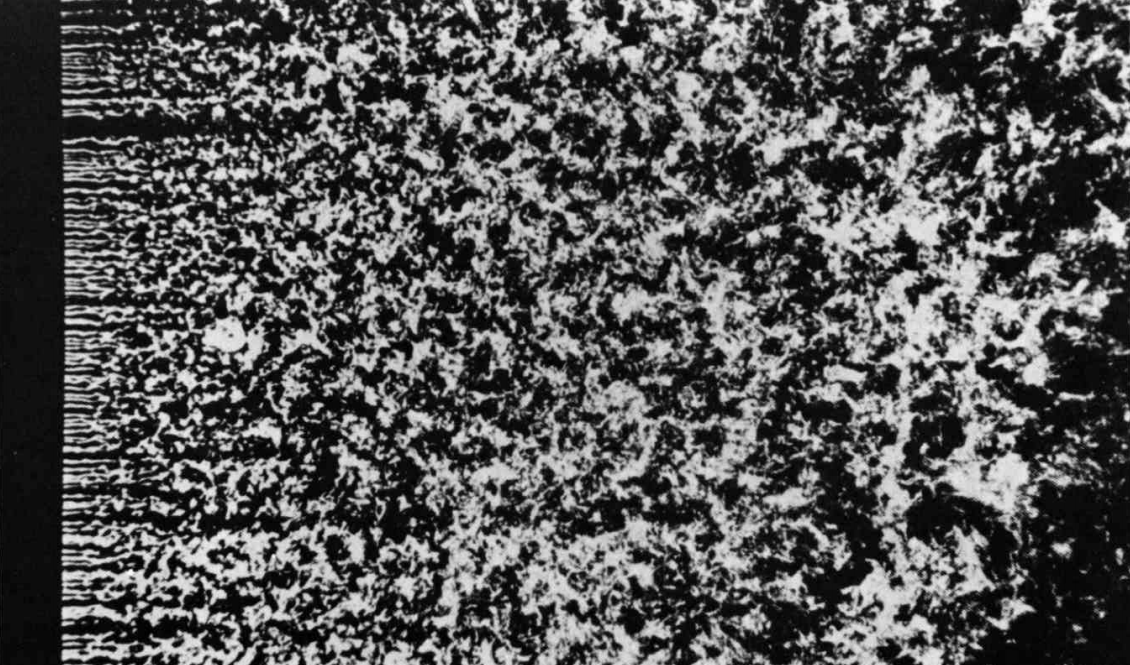
\includegraphics[width=\textwidth]{./Abbildungen/TurbulentMotion_Introduction.png}
  \captionsetup{width=0.97\linewidth}
	\caption{Photograph courtesy of Hassan Nagib and Thomas Corke. Formation of a nearly isotropic turbulent flow field behind a grid \cite{albumOfFluidMotion}.}
	\label{introduction_picture}
\end{figure}
Particle-laden turbulent flows are ubiquitous in nature.
Spray automization in fuel injectors, cyclonic particle separation in oil refineries and sediment accumulation in pipelines are examples for technical applications, where it is of huge interest to predict the impact of the particles on turbulent flows.
Turbulence augmentation or attenuation by particles is therefore a decisive factor.
\newline
A study about the impact of particles on the isotropic decaying turbulent flow is presented.
Incompressible, isothermal and isotropic decaying turbulence will serve as the carrier flow. Gravity is omitted to avoid prominent directions. Isotropic turbulence is a relatively good assumption when a small region of a high-Reynolds-number flow, which is not affected by boundary effects, is observed \cite{Kolmogorov1941}. This fact is visualized by Fig \ref{introduction_picture}. Describing turbulent flows is a large task because of the involvement of many different scales of turbulent motion.
\newline
In this work the influence of the particles on the isotropic decaying turbulence is numerically calculated by using direct numerical (DNS) and large-eddy simulations (LES). Direct numerical simulations are able to resolve all scales of turbulent motion due to their high grid refinement. Large-eddy simulations have a lower grid resolution and use therefore a subgrid-scale model (SGS) to model these scales. This type of simulation therefore has a lower computational effort.
\newline
The simulations were carried out using the point-particle approach, where each particle is tracked via a Langrangian approach. The feedback of the particles on the flow field is modeled by sources and sinks, which is referred to as two-way coupling. Alternatives are one-way coupling, at which only the flow exert influence on the particles, and four-way coupling, which extends two-way coupling by particle-particle interactions. Two-way coupling is fitting for the simulations in this study, because the volume fraction $\phi_\mathrm{v}= 10^{-3}$ of the particles is large enough to alter the turbulence. Volume fractions below $\phi_\mathrm{v}= 10^{-6}$ are referred to as one-way coupling and the interactions that can be observed at values greater than $\phi_\mathrm{v}= 10^{-3}$ are called four-way coupling \cite{particleladenTurbulentFlows:DirectSimulationAndClosureModels}\cite{OnPredictingParticle-LadenTurbulentFlows}.
The particle diameter is defined to be smaller than the Kolmogorov scale, i.e. the smallest scale of the turbulent flow. The particle density is much higher than the fluid density.
\newline
To lower the computational effort in general, a new variable, which describes the fraction of physical to numerical point particles, is introduced and validated.
\newline
The structure of this work is described in the following. 
First, mathematical models for single-phase and particle dynamics are given. 
Additionally, the scales of turbulent motion are described.
Thereafter, the computational basics of both DNS and LES and their respective advantages and disadvantages are explained.
Subsequently, the used discretization method to integrate the particle tracking equations is described and the 'computational point particles', in the following referred to as CPP, are introduced. 
The CPP approach is validated by analyzing turbulent kinetic energy budgets for LES and DNS.
Also the number of particles that is needed to get consistent average values for the flow characteristics is investigated.
Finally, a short conclusion is given.
\pagebreak
\section{Mathematical models}
To provide a common basis of knowledge, the basic equations and scales of a flow are introduced, as well as particle-considering equations.
\newline
\subsection{Equations governing the fluid phase}
The conservation of mass, momentum and energy for a control volume reads
\begin{equation}
  \int\limits_V \frac{\partial{\vec{Q}}}{\partial{t}} \, \mathrm{d} V+ \int\limits_{\partial{V}} \vec{\bar{H}} \cdot \vec{n} \, \mathrm{d} A = \vec0
\end{equation}
with time $t$ and the flux tensor $ \vec{\bar{H}} $.
The vector $ \vec{Q} $ contains the variables fluid density $ \rho $, 
fluid velocity $ \vec{u} $ and specific inner energy $ E $: 
\begin{equation}
 \vec{Q}= \left( \begin{array}{c}\rho\\\rho \vec{u}\\\rho E \end{array} \right).
\end{equation}
$\vec{\bar{H}} $ is the flux tensor which contains the inviscid and viscous flux, i.e.
\begin{equation} \label{NavierStokes}
\vec{\bar{H}} = \vec{\bar{H}^\mathrm{i}} + \vec{\bar{H}^\mathrm{v}} = 
 \left( \begin{array}{c}\rho \vec{u}\\\rho \vec{u} \vec{u} + p\\\vec{u} (\rho E + p) \end{array} \right) - 
 \frac{1}{Re} \left( \begin{array}{c}\ 0 \\ \matrix{\bar{\tau}}\\ \matrix{\bar{\tau}} \vec{u} + \vec{q} \end{array} \right).
\end{equation} 
$ \vec{\bar{H}^\mathrm{i}} $ contains the variables that are independent of the fluid's viscosity and $ \vec{\bar{H}^\mathrm{v}} $ represents the effects of viscosity, with shear stress $\matrix{\bar{\tau}}$ and heat conduction $\vec{q}$. The Reynolds number 
$ Re = \frac{\rho v d}{\mu} $ is defined to be the ratio of inertia forces to viscous forces. This is also due to the 
fact that two familiar objects with Re being identical behave similar in flows.
To solve the Navier-Stokes equations, more information regarding some variables is required. For calculating the specific inner energy $ E $ 
and the heat conduction $ \vec{q} $, the following equations are used
\begin{equation}
 E = e  \frac{1}{2} \vec{|u|}^2,
\end{equation}
\begin{equation}
 \vec{q} = - \frac{\mu}{Pr (\gamma - 1)} \vec\nabla T,
\end{equation}
with 
\begin{equation}
 \gamma = \frac{c_p}{c_v}
\end{equation}
and the Prandtl number
$ Pr = \frac{\mu_\infty c_\mathrm{p}}{k_\mathrm{t}}$
using the specific heat capacities of the fluid $ c_\mathrm{v} $ and $ c_\mathrm{p} $.
Assuming that the fluid is a newtonian fluid, the linear correlation between the stress and the rate of strain results in:
\begin{equation}
 \matrix{\bar{\tau}} = 2 \mu \matrix{\bar{S}} - \frac{2}{3} \mu (\vec\nabla \cdot \vec{u}) \matrix{\bar{I}},
\end{equation}
in which $ \matrix{\bar{S}} = \frac{(\vec\nabla \vec{u})(\vec\nabla \vec{u})^T}{2} $ denotes the rate-of-strain tensor. Additionally, the viscosity
$ \mu $ can be approximated by Sutherland's law
\begin{equation}
 \mu (T) = \mu_\infty \biggl(\frac{T}{t_\infty}\biggl)^{3/2} \frac{T_\infty + S}{T + S},
\end{equation}
where S is the Sutherland temperature. Sutherland's law is based on the ideal gas theory.
To achieve closure the caloric state equation $ e = c_\mathrm{v} T $ and the state equation for an ideal gas $
p = \rho R T $ are used. The specific gas constant is determined by $ R = c_\mathrm{p} - c_\mathrm{v} $. 
\newline
\subsection{Scales of turbulent flows}
Turbulent flows contain eddies, which are the reverse currents in the flow, of all sizes and shapes. Large-scale eddies bring energy to the flow, which is then passed down to smaller scales, and finally dissipated into heat by viscous effects. This behavior is called the 'energy cascade' and was first described by Richardson in the year 1920 \cite{Richardson1920}. The theory then was quantified by Kolmogorov \cite{Kolmogorov1941}.
\newline
The first set of scales describe the large eddies. At these scales the energy is brought into the flow, creating the 'energy-containing range'. The corresponding timescale, which is most times called 'eddy turnover time', is defined as
\begin{equation}
\tau_\mathrm{L} = \frac{L}{U},
\end{equation}
with the integral length scale $L$ (\ref{eq:integralLengthScale}) and the characteristic fluid velocity $U$.
\newline
The smallest scales in a turbulent flow are the Kolmogorov length $\eta$ and time scale $\tau_\mathrm{\eta}$. At these scales, the effects of viscosity take place and the energy dissipates into heat. With the estimate $\epsilon \approx \frac{U^3}{L} $ they can be written as
\begin{equation}
\eta = \biggl (\frac{\nu^3 L}{U^3} \biggl )^{1/4}
\end{equation}
and
\begin{equation}
\tau_\mathrm{\eta} = \biggl (\frac{\nu L}{U^3} \biggl ).
\end{equation}
Both these scales are coupled by the Reynolds numbers
\begin{equation}
\frac{L}{\eta} = Re^{3/4}
\end{equation}
and
\begin{equation}
\frac{\tau_\mathrm{L}}{\tau_\mathrm{\eta}} = {Re_\mathrm{L}}^{1/2}.
\end{equation}
It can be observed from these equations that the spacing between the scales increases for higher Reynolds numbers. 
\newline
Characteristic length scales $\lambda$ and $L$ of a turbulent flow can be defined by the two-point correlation $R$, which is the normalized product of the velocity's fluctuation $\vec{u'}$ at two different positions 
$\vec{x}$ and $\vec{x} + \vec{r}$ at the same time $t$
\begin{equation}
R (\vec{x}, \vec{r}) = \frac{\overline{\vec{u'}(\vec{x}, t)\vec{u'}(\vec{x} + \vec{r}, t)}}{\sqrt{\overline{\vec{u'}^2(\vec{x}, t)}}\sqrt{\overline{\vec{u'}^2(\vec{x} + \vec{r}, t)}}},
\end{equation}
as
\begin{equation}
 \frac{1}{\lambda^2} = -\frac{1}{2}\biggl(\frac{\partial^2 R}{\partial \vec{r}^2}\biggl),
\end{equation}
\begin{equation}
\lambda = \sqrt{15 \frac{\nu}{\epsilon}} |\vec{u'}|
\end{equation}
or
\begin{equation} \label{eq:integralLengthScale}
L = \int_{0}^{\infty} R (\vec{x}, \vec{r})  \, \mathrm{d}\vec{r}
\end{equation}
with $\lambda$ being the Taylor microscale, $L$ the integral length scale and $|\vec{u'}|$ denoting the absolute value of the velocity's fluctuation.
\newline
The Taylor microscale can be used to compute the Taylor-scale Reynolds number
\begin{equation}
Re_\mathrm{\lambda} = \frac{|\vec{u'}| \lambda}{\nu}.
\end{equation}
\newline
\subsection{Particle dynamics} %Steffen
To take the forces acting from the particles on the fluid into account the Navier-Stokes equation for the carrier fluid \eqref{NavierStokes} is extended by the force $\vec{F}$ that acts on the ambient cells with different intensity regarding on the distance between these cells and the particle
\begin{equation}
\vec{F} = \vec{F}_\mathrm{pp} \cdot \frac{\mathrm{e}^{- \big(d_\mathrm{i}^\mathrm{2}/(\sigma \Delta^\mathrm{2})\big)}}{\sum \limits_{i} e^{- \big(d_\mathrm{i}^\mathrm{2}/(\sigma \Delta^\mathrm{2}) \big)}},
\end{equation}
with the distance between particle postion and midpoint of the cell $d_\mathrm{i}$, the length of the cells $\Delta$ and a smoothing parameter $\sigma$ that controls the distribution of $\vec{F}$ on the adjacent cells.
$\vec{F}_\mathrm{pp}$ is the sum of pressure and shear forces acting on the particles and is described explicitly in the Maxey-Riley equation that can be achieved from \cite{EquationOfMotionForASmallRigidSphereInANonuniformFlow}.
$\vec{F}_\mathrm{pp}$ can be divided into several forces. 
Reduced to the governing forces acting on the particles and with neglection of gravity the dynamic equation of the particles becomes
\begin{multline} \label{navier_stokes_particle}
\\ \vec{F}_\mathrm{pp} = m_\mathrm{p} \frac{\mathrm{d}\vec{v}_\mathrm{p}}{\mathrm{d}t} =\rho V_\mathrm{p}\frac{\mathrm{D}\vec{u}}{\mathrm{D}t} -\frac{3}{4}\rho \mathrm{V}_\mathrm{p} \frac{C_\mathrm{d}}{d_\mathrm{p}}|\vec{v}_\mathrm{p}-\vec{u}|(\vec{v}_\mathrm{p}-\vec{u})+ \frac{1}{2}\rho \mathrm{V}_\mathrm{p} \biggl(\frac{\mathrm{D}\vec{u}}{\mathrm{D}t}-\frac{\mathrm{d}\vec{v}_\mathrm{p}}{\mathrm{d}t}\biggl) + 
\\ \frac{3}{2}d_\mathrm{p}^\mathrm{2}\rho\sqrt{\pi\nu}\int_{t_\mathrm{0}}^{t} \frac{\mathrm{d}t'}{(t-t')^\mathrm{1/2}} \biggl(\frac{\mathrm{D}\vec{u}}{\mathrm{D}t'}- \frac{\mathrm{d}\vec{v}_\mathrm{p}}{\mathrm{d}t'}\biggl).
\end{multline}
$\vec{v}_\mathrm{p}(\vec{x}_\mathrm{p},t)$ is the particle velocity vector with the time derivative $\mathrm{d}/\mathrm{d}t$ following a sphere while $\mathrm{D}/\mathrm{D}t$  is the time derivative following a fluid unit. 
The individual forces on the right side of the equation are stated in the following:
\begin{itemize} 
\item  $\rho V_\mathrm{p}\frac{\mathrm{D}\vec{u}}{\mathrm{D}t}$: \newline
pressure gradient of the undisturbed flow
\item  $-\frac{3}{4}\rho \mathrm{V}_\mathrm{p} \frac{C_\mathrm{d}}{d_\mathrm{p}}|\vec{v}_\mathrm{p}-    \vec{u}|(\vec{v}_\mathrm{p}-\vec{u})$:\newline
hydrodynamical drag force that is parallel to the undisturbed streamlines, which depends on an empirical drag coefficient $C_{\mathrm{d}}$ defined by Schiller and Naumann as
$C_\mathrm{d} = \frac{24}{Re_\mathrm{p}}(1+0.15Re_\mathrm{p}^\mathrm{0.687})$.
It is described by the Stokes' law as the force of viscosity acting on the interface of small spherical particles and fluid that can be achieved at very low Reynolds numbers in a viscous fluid

\item $\frac{1}{2}\rho \mathrm{V}_\mathrm{p} \biggl(\frac{\mathrm{D}\vec{u}}{\mathrm{D}t}-\frac{\mathrm{d}\vec{v}_\mathrm{p}}{\mathrm{d}t}\biggl)$:\newline
added mass force, representing the influence of the fluid's inertia that has an impact on the particle, in case of a different acceleration than the particles
\item $\frac{3}{2}d_\mathrm{p}^\mathrm{2}\rho\sqrt{\pi\nu}\int_{t_\mathrm{0}}^{t} \frac{\mathrm{d}t'}{(t-t')^\mathrm{1/2}} \biggl(\frac{\mathrm{D}\vec{u}}{\mathrm{D}t'}- \frac{\mathrm{d}\vec{v}_\mathrm{p}}{\mathrm{d}t'}\biggl) $: \newline
history force taking diffusion and convection into account that results from vortices in the slipstream of the particles
\end{itemize}

As presented by Vincenzo Armenio and Virgilio Fiorotto \cite{TheImportanceOfTheFocusActingOnParticlesInTurbulentFlows} compared to the Stokes drag all other forces could be neglected with rising particle density, so due to the density ratio being $\rho_\mathrm{p}/\rho \gg 1$, $\vec{F}_\mathrm{pp}$ can be approximately reduced to the dominating viscous drag. \eqref{navier_stokes_particle} becomes 
\begin{equation} \label{kurze_Partikelgleichung}
\vec{F}_\mathrm{pp} =  m_\mathrm{p} \frac{\mathrm{d}\vec{v}_\mathrm{p}}{\mathrm{d}t} = \frac{3}{4}\rho \mathrm{V}_\mathrm{p} \frac{C_\mathrm{d}}{d_\mathrm{p}}|\vec{v}_\mathrm{p}-\vec{u}|(\vec{v}_\mathrm{p}-\vec{u}).
\end{equation} 
Using the particle Reynolds number $Re_\mathrm{p} = \frac{v_\mathrm{r}d_\mathrm{p}}{\nu}$ with the relative velocity between particle and fluid $v_\mathrm{r}$,  \eqref{kurze_Partikelgleichung} can be compressed, which is described in detail in \cite{computationalMethodsforMultiphaseFlow}.
\begin{equation} \label{shortPaticleDynamics}
\rho_\mathrm{p}\frac{\mathrm{d}\vec{v}_\mathrm{p}}{\mathrm{d}t} = \rho_\mathrm{p}\frac{\vec{v}_\mathrm{p}-\vec{u}}{\tau_\mathrm{p}}f_\mathrm{d}.
\end{equation}
Here the particle response time $\tau_\mathrm{p} = \frac{(\rho_\mathrm{p}/\rho)d_\mathrm{p}^\mathrm{2}}{18\nu}$ is introduced which is a time constant in the exponential decay of the particle velocity as a result of an upcoming fluid drag and physically represents the time scale over which the drag force decreases the particle's relative velocity to zero.
$f_\mathrm{d} = 1+0.15Re_\mathrm{p}^\mathrm{0.687}$ is a correction factor depending on the flow conditions.
Together with the kinematic equation of a particle   
\begin{equation}
 \frac{\mathrm{d}\vec{x}_\mathrm{p}}{\mathrm{d}t} = \vec{v}_\mathrm{p},
\end{equation}
the adjusted equation \eqref{NavierStokes} and \eqref{shortPaticleDynamics} form the basic equations for the particle laden system. 
\pagebreak
\section{Numerical methods} %Julian
Two numerical methods are discussed and their main differences pointed out in the following chapter, the DNS (direct numerical simulation) and the LES (large-eddy simulation). The basis of both are the Navier-Stokes equations as described above.
\newline
\subsection{Discretization of the particle dynamics}
To integrate the Lagrangian particle tracking equations, discussed before, a predictor-corrector scheme based on the trapezoidal rule for numerical integration
\begin{equation}
f (t + \delta t) \approx f(t) + \frac{\delta t}{2} \left[ \frac{\partial f(t)}{\partial t} + \frac{\partial f(t + \delta t)}{\partial t} \right ]
\end{equation}
is used.
\newline
The first step is the prediction of the new particle position $\vec{x}_{\mathrm{p}, n+1}$ using a Taylor expansion for a small time step $\delta t$
\begin{equation}
\vec{x}_{\mathrm{p}, n+1} = \vec{x}_{\mathrm{p}, n} + \delta t \vec{v}_{\mathrm{p}, n} + \frac{1}{2} \delta t^2 \vec{a}_{\mathrm{p}, n},
\end{equation}
with $\vec{a}_{\mathrm{p}, n}$ particle acceleration. 
\newline
To avoid filtering effects, the fluid velocity $\vec{u}(\vec{x}_{\mathrm{p}, n+1})$ at the particle position $\vec{x}_{\mathrm{p}, n+1}$ is set equal to the nearest cell fluid velocity. 
\newline
The updated velocity and acceleration are calculated as
\begin{equation}
\vec{v}_{\mathrm{p}, n+1} = \frac{\vec{v}_{\mathrm{p}, n} + \frac{1}{2} \delta t \left(\vec{a}_{\mathrm{p}, }n + \frac{f_\mathrm{d}}{\tau_\mathrm{p}}\vec{u}(\vec{x}_{\mathrm{p}, n+1}) \right)}{1 + \frac{1}{2} \frac{f_\mathrm{D}}{\tau_\mathrm{p}} \delta t},
\end{equation}
\begin{equation}
\vec{a}_{\mathrm{p}, n+1} = \frac{\frac{f_\mathrm{D}}{\tau_\mathrm{p}} \left(\vec{u}(\vec{x}_{\mathrm{p}, n+1}) - \vec{v}_{\mathrm{p}, n} - \frac{1}{2} \delta t \vec{a}_{\mathrm{p}, n} \right)}{1 + \frac{1}{2} \frac{f_\mathrm{D}}{\tau_\mathrm{p}} \delta t}.
\end{equation}
The updated particle position must be corrected by an additional term according to the trapezoidal rule
\begin{equation}
\vec{x}_{\mathrm{p}, n+1} = \vec{x}_{\mathrm{p}, n} + \frac{1}{2} \delta t \left( \vec{v}_{\mathrm{p}, n+1} + \vec{v}_{\mathrm{p}, n} \right) + \frac{1}{12} \delta t^2 \left( \vec{a}_{\mathrm{p}, n+1} - \vec{a}_{\mathrm{p}, n} \right).
\end{equation}
\newline
\subsection{Direct numerical simulation}
With DNS, the Navier-Stokes equations are solved completely. This provides a very accurate result, as all scales of motion are being resolved. Still it requires an immense level of computational resources which increases rapidly with the Reynolds number: $N^3 \propto 4.4 Re_{\mathrm{L}}^{9/4} \approx 0.06 Re_{\mathrm{\lambda}}^{9/2}$ with gridsize N of the simulation. These computational resources were not available until the 1970s. With the LES, as described below, the computational effort is 99.98 \% less compared to DNS, which indeed is the fraction of the dissipative scale. This leaves 0.02 \% of the flow, which is correlative with the fraction of the energy-containing larger-scale \cite{turbulentFlows}.
\newline
\subsection{Large-eddy simulation}
\begin{figure}[h]
    \centering
    \begin{minipage}[t]{.5\textwidth}
        \centering
        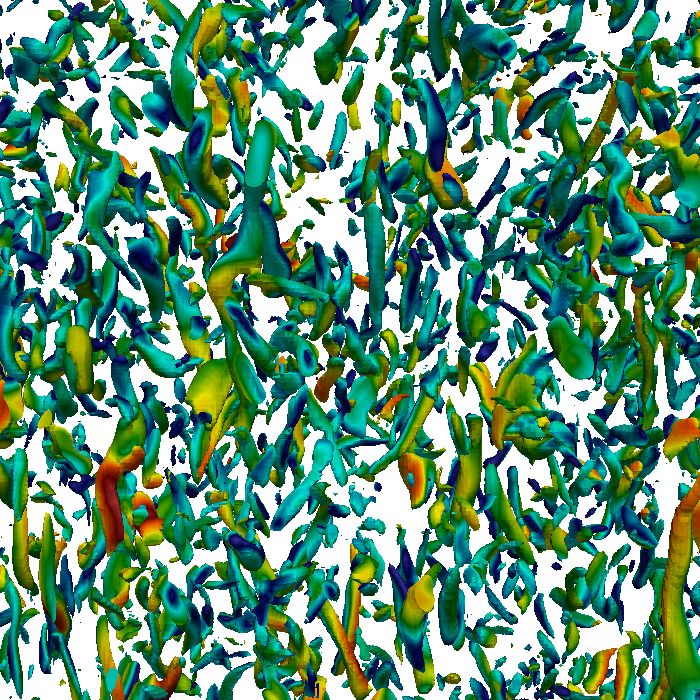
\includegraphics[width=0.95\linewidth]{./Abbildungen/256_velocity_4.png}
        \label{256_velocity}
    \end{minipage}%
    \begin{minipage}[t]{0.5\textwidth}
        \centering
        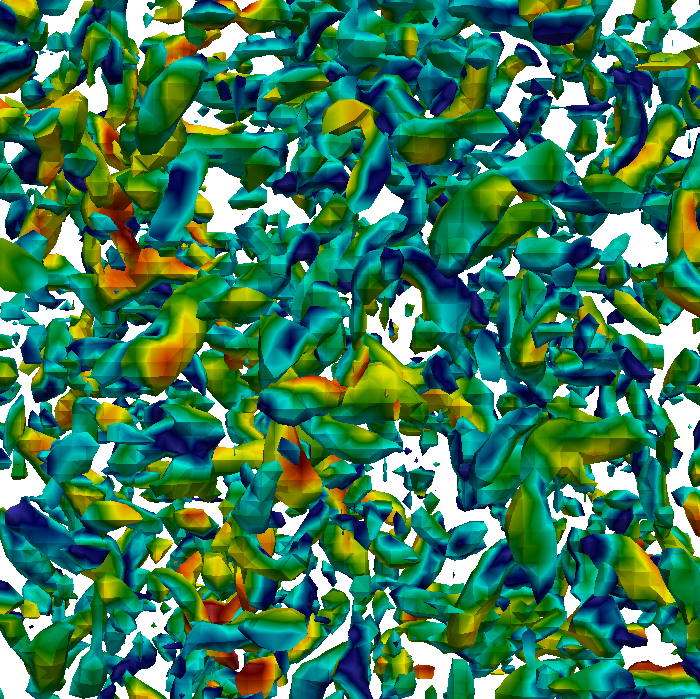
\includegraphics[width=0.95\linewidth]{./Abbildungen/64_velocity.png}
        \label{64_velocity}
    \end{minipage}
    \captionsetup{width=0.97\linewidth}
\caption{Comparison between DNS and LES. 'Worm-like' structures in an isotropic flow field simulated in different grid resolutions. The more refined grid on the left show more and better resolved structures, while the right picture reveals more artificially generated artifacts. For creation see Appendix A.}
\end{figure}
Due to the fact that DNS is effortful, LES was created to save time and resources. The energy containing larger-scale motion is completely resolved and the small effects of the smaller-scale motion are modeled. Otherwise in DNS resolving the small dissipative scale would require most of the computational resources.
\newline
Simulating only the larger-scale motions is called filtering, which means that the smaller-scale motions, also known as fluctuation, are filtered out. The filtered velocity field is calculated by $\bar U(\vec{x}) = \int_{-\infty}^{\infty} G(\vec{r})U(\vec{x} - \vec{r})  \, \mathrm{d}\vec{r}$, with $G(\vec{r}) $ being a homogeneous filter function. For further information on filter functions, the works of Pope \cite{turbulentFlows} should be considered. To model the filtered smaller-scale motions usually a subgrid-scale (SGS) model is used. According to Hickel (2007) the interference between explicit SGS and the truncation error can be exploited, i.e. the truncation error can serve as model of the effects of unresolved scales, which is therefore an implicit SGS model. Thus it is called implicit LES (ILES) \cite{implicitLES}. 
\subsection{Computational point particles}
The high number of point particles requires even more computational resources for the particle-laden simulations than for the single-phase simulations. The idea to reduce this requirement is to create clusters of point particles. For this purpose the ratio $\lambda_\mathrm{c}$ of physical point particles $N_\mathrm{p}$ to CPPs $N_\mathrm{c}$ is introduced ($\lambda_\mathrm{c} = \frac{N_\mathrm{p}}{N_\mathrm{c}}$). To compensate this lack of particles, the coupling force is multiplied by $\lambda_\mathrm{c}$, due to the $\lambda_\mathrm{c}$-fold mass of the (cluster-)particles.
\newline
\subsection{Applied simulation}
The simulations were carried out using ZFS, the simulation tool developed and implemented at the Institute of Aerodynamics at RWTH Aachen University 
\cite{anAdaptiveMultilevelMultigridFormulationForCartesianHierarchicalGridMethods} \cite{aStrictlyConservativeCartesianCutCellMethodForCompressibleViscousFlowsOnAdaptiveGrids}. 
The tool is capable of simulating finite-volume flows of compressible fluids. In the simulations, which results the reader can see at hand, the Mach-number $Ma$ was set to 0.1 to simulate an almost incompressible fluid.
\pagebreak
\section{Results}
In this section the properties and results of the simulations that have been carried out will be presented. Special emphasis will be put on the turbulent kinetic energy budgets and their use to interpret the findings.
\newline
\subsection{Simulation properties}
All cases were simulated on a cubic domain and a cartesian grid using multiple grid refinement levels, $64^3$, $96^3$ and $128^3$ representing the LES hence the need to model smaller scales with SGS-models is present. Due to higher grid refinement in the $256^3$-case, these smaller scales can be directly simulated and therefore this simulation is a DNS.
\newline
The particle-free case was initialized using a seed-based random generator. At the time normalized by eddy turnover time $t^* \approx 0.27$ a restart file is written out to initialize the subsequent simulation of the particle-laden isotropic turbulence. This file is then used to set up a second simulation including particle load. Both these cases, DNSs of a single-phase and a particle-laden flow will be used as reference for analyzing other results. Single-phase simulations will in the following be referred to as sP, and particle-laden ones as PP. The PP simulation was set up to match the volume fraction $\phi_\mathrm{v}= 10^{-3}$ and mass fraction of $\phi_\mathrm{m}=1$. Both were constant in all simulations regarding CPPs. The ratio of the densities for this set of simulations was set to $\frac{\rho_\mathrm{p}}{\rho} = 1000$, the particle diameter is matched by $d_\mathrm{p} \approx 0.6 \eta$. In this work a smoothing parameter $\sigma$ of 4 was used. The injection of a million spherical point-particles was carried out interpolating the velocities of the surrounding fluid. At the timestep of injection the particle response time $\tau_\mathrm{p}$ was 0.03497, the Prandtl number was 0.72 and $Re_\lambda$ was 57.9757. 
\newline
\subsection{The turbulent kinetic energy budget}
The change in kinetic energy of the fluid in particle-laden decaying isotropic turbulence is determined by the coupling rate $\Psi$, which describes the energy transfer between both fluid and particle phase $\frac{\partial E_\mathrm{k}}{\partial t}$, and the integral dissipation rate $\vec{\varepsilon}$:
\begin{equation}
\frac{\partial E_\mathrm{k}}{\partial t} = \Psi_\mathrm{pp} (t) - \vec{\varepsilon} (t).
\end{equation}
As mentioned before, the flow field is considered nearly incompressible, therefore the equation  for the viscous dissipation rate can be approximated by
\begin{equation}
 \epsilon (t) \approx 2 \mu \vec{\bar{S}}\vec{:}\vec{\bar{S}},
\end{equation}
where $\vec{:}$ denotes the inner tensor product. This rate can then be integrated over the full fluid domain $\Upsilon_\mathrm{f}$, leading to 
\begin{equation}
\varepsilon (t) = \int\limits_{\Upsilon_\mathrm{f}} \epsilon(t) \mathrm{d}V.
\end{equation}
As the dissipation rate is always of positive value, it acts as a sink for the fluid's turbulent kinetic energy. In difference to that, the coupling rate can serve either as source or sink, depending on the acceleration of the particles \cite{mechanismsoftwowaycoupling}. The coupling rate for fully resolved particles is defined as
\begin{equation}
\Psi (t) = \sum_{p=1}^{N_\mathrm{p}} \Psi_\mathrm{p}= - \sum_{p=1}^{N_\mathrm{p}} (\vec{F}_\mathrm{p} \cdot \vec{v}_\mathrm{p} + \vec{T}_\mathrm{p} \cdot \vec{\omega}_\mathrm{p}),
\end{equation}
using surface force $\vec{F}_\mathrm{p}$, particle velocity $\vec{v}_\mathrm{p}$, torque $\vec{T}_\mathrm{p}$ and angular velocity $\vec{\omega}_\mathrm{p}$ to describe the transfer of kinetic energy resulting at each particle. The torque can be neglected for the used point-particle approach.
\begin{equation}
\frac{\mathrm{d}E_\mathrm{kB}}{\mathrm{d}t} = - \Psi (t)
\end{equation}
therefore is the rate of change for the global kinetic energy of the particles.
Additionally the particles change the fluid's rate of dissipation $\vec{\varepsilon}$ due to their volume forces. 
Schneiders et al. \cite{schneiders2017} therefore proposed a separation of dissipation rates for suspended heavy particles
\begin{equation}
\frac{\partial E_\mathrm{k}}{\partial t} = \Psi (t) - \vec{\bar{\varepsilon}} (t) - \vec{\varepsilon}' (t).
\end{equation}
In this equation, $\vec{\bar{\varepsilon}} (t)$ displays the dissipation rate of the flow field and $\vec{\varepsilon}' (t)$ is the additional dissipation rate introduced by the injected point-particles. For $\rho_\mathrm{p} \gg \rho$ and the point-particle approach the coupling rate $\Psi$ and the additional dissipation rate $\vec{\varepsilon}'$ are implicitly coupled
\begin{equation}
\Psi_\mathrm{pp} (t) = \Psi -\vec{\varepsilon}'.
\end{equation}
The additional dissipation rate for fully resolved particles can be computed by
\begin{equation}
	\vec{\varepsilon}' = \sum_{p=1}^{N_\mathrm{p}} \vec{F}_\mathrm{p} \cdot (\vec{u}_\mathrm{p}-\vec{v}_\mathrm{p}),
\end{equation}
using the velocity of the fluid $\vec{u}_\mathrm{p}$ at the particle position.
The coupling rate in the special case of point particles then simplifies to 
\begin{equation}
\Psi_\mathrm{pp} (t) = - \sum_{p=1}^{N_\mathrm{p}} \vec{F}_\mathrm{p} \cdot \vec{u}_\mathrm{p}.
\end{equation}
\newline
\subsection{Simulation results}
\begin{figure}[h]
    \centering
    \begin{minipage}{0.5\textwidth}
        \centering
 	   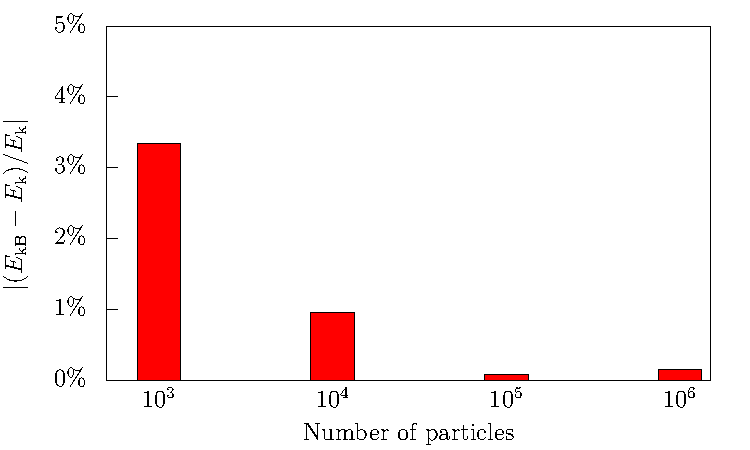
\includegraphics[width=\linewidth]{./Abbildungen/kineticEnergy_numberOfParticles.pdf}
    \end{minipage}%
        \begin{minipage}{0.5\textwidth}
        \centering
        \caption{Initializing different numbers of point-particles on a $128^3$-grid. An inaccuracy can be observed for small numbers of particles. This behavior can be observed for all other resolutions.}
	\label{kineticEnergy_numberofparticles}
    \end{minipage}
    \end{figure}
The first set of simulation was set up to investigate how different numbers of injected particles have an influence on the difference of turbulent kinetic energy of both particle and fluid. As mathematical description of turbulent flows is based on statistics, small numbers of particles can lead to questionable results. An example for the deviation in kinetic energy for different numbers of particles can be found in Fig. \ref{kineticEnergy_numberofparticles}. The normalized difference in kinetic energy $E_\mathrm{kB}$ of the particles and the flow itself $E_\mathrm{k}$ shows a correlation between particle number and accuracy in in this single simulation. Although this was just a single initialization of particles in a flow, it can be stated that simulations using only $10^3$ or even up to $10^4$ particles are not accurate enough for technical or scientific use of data. Simulations in other grid sizes show similar results.
\begin{figure}[h]
    \centering
    \begin{minipage}[t]{0.5\textwidth}
        \centering
 	   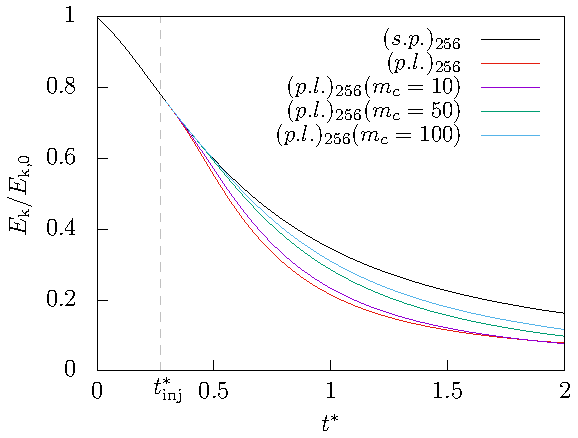
\includegraphics[width=\linewidth]{./Abbildungen/256/kineticEnergy_time.pdf}
	   \caption{Kinetic energy $E_\mathrm{k}$ normalized by its initial value $E_\mathrm{k,0}$ over time normalized by initial eddy turnover time. Shortly after the injection the PP-cases separates from the sP-flow. The higher-clustered cases show less distinctions from the sP-case.}
	\label{kineticEnergy_time_256}
    \end{minipage}%
\begin{minipage}[t]{0.5\textwidth}
        \centering
        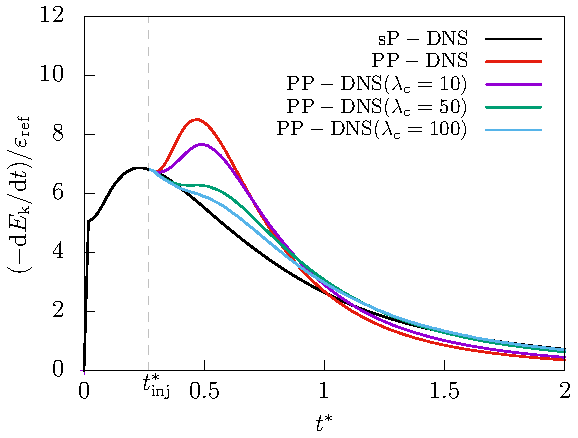
\includegraphics[width=\linewidth]{./Abbildungen/256/der(kineticEnergy)_time.pdf}
        \caption{Change in kinetic energy over time normalized by initial eddy turnover time. After $t^* \approx 1$ the unclustered PP-case shows a lower decay rate in kinetic energy than the sP-case.}
        \label{der_kineticEnergy_256}
    \end{minipage}
\end{figure}
\newline
The second set of simulations conducted in this work is set up to investigate the influence of CPPs on the accuracy of the simulations with the goal to minimize computational effort, while still achieving high quality results. For this purpose, the variable $\lambda_\mathrm{c}$, which was established before, was implemented in the program code. The simulations were then set up with the overall same number of a million particles, altering just $\lambda_\mathrm{c}$. It can be seen in Fig. \ref{kineticEnergy_time_256} and \ref{der_kineticEnergy_256} that the decay in kinetic energy from the injection point depends highly on the number of clustered particles. It can be stated that the flow's statistics for high $\lambda_\mathrm{c}$ converge towards the sP-case. 
\begin{figure}[h]
    \centering
    \begin{minipage}[t]{0.5\textwidth}
         \centering
        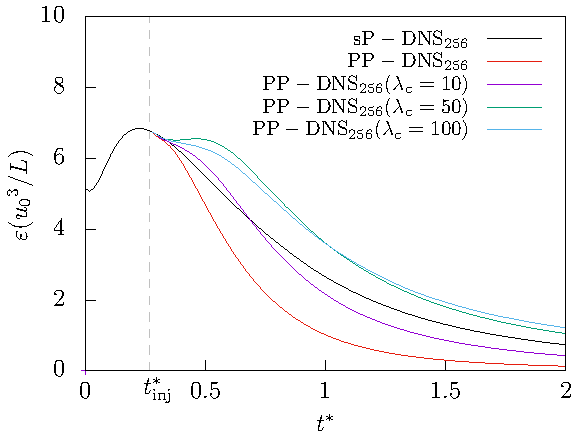
\includegraphics[width=\linewidth]{./Abbildungen/256/diss_time.pdf}
        \caption{Normalized dissipation rate $\bar{\vec{\varepsilon}}$ over time normalized by initial eddy turnover time. The unclustered PP-case shows a lower dissipation rate than the sP-case. Highly clustered PP-cases show a higher dissipation rate.}
        \label{diss_time_256}
    \end{minipage}%
    \begin{minipage}[t]{0.5\textwidth}
        \centering
        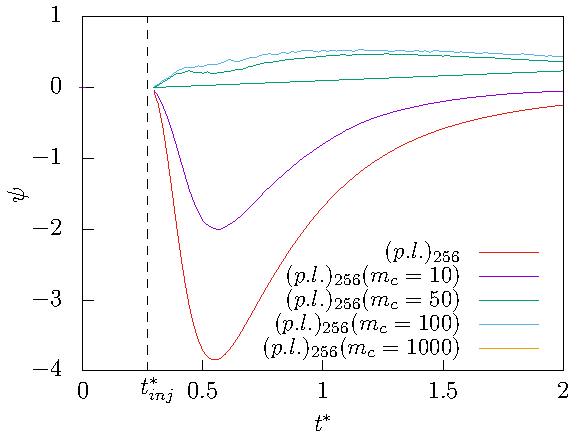
\includegraphics[width=\linewidth]{./Abbildungen/256/coupling_time.pdf}
        \caption{Normalized point-particle coupling rate $\Psi_\mathrm{pp}$ over time normalized by initial eddy turnover time. The PP-case without clustering shows the lowest coupling rate. Both highly-clustered PP-cases show physically questionable behavior.}
        \label{coupling_time_256}
    \end{minipage}
\end{figure}
\newline
Fig. \ref{diss_time_256} and \ref{coupling_time_256} can be interpreted using the turbulent kinetic energy budget introduced earlier. The PP-case without clustering shows a lower dissipation rate than the sP-case, both highly-clustered cases show a higher rate over the monitored period of time, which is an unphysical behavior. The coupling rate is negative the whole time for the PP-cases with lower $\lambda_\mathrm{c}$ and positive for the higher-clustered cases. Both these effects form the change in kinetic energy in particle-laden isotropic flow found in Fig. \ref{der_kineticEnergy_256}.
\newline
Being very similar in the time shortly after the injection, the flow statistics diverge for different $\lambda_\mathrm{c}$ rapidly. The variables of these simulations one turnover time after the injection can be found in table \ref{table_values}. 
\begin{table}[h]
	\begin{center}
	\begin{tabular}{l l | c c c c c c }
	$\lambda_\mathrm{c}$& $\frac{m_\mathrm{c}}{m_\mathrm{V,cell}}$ & $\epsilon \frac{{u_0}^3}{L}$ & $\frac{\lambda}{L}$ & $\frac{\eta}{L} $ & $Re_\lambda$ \\
	\hline
	\hline
	1 &16.78 & 0.97& 0.039 & 0.0032 & 38.73 &\\
	10 &167.78 & 2.08 & 0.028 & 0.0026 & 28.66 &\\
	50 &838.86 & 3.51 & 0.024 & 0.0023 & 27.31 &\\
	100 &1677.72 & 3.51 & 0.025 & 0.0023 & 29.42 &\\
	\hline
	\end{tabular}
	\captionsetup{width=0.9\linewidth}
	\caption{Variables of the first set of simulations one turnover time after injection for the $256^3$-case}
	\label{table_values}
	\end{center}
	\end{table}
In Fig. \ref{particlekineticenergy_time_256} the kinetic energy of the particles is displayed. As $\lambda_\mathrm{c}$ rises, the decay in the kinetic energy of the particles becomes smaller. This behavior leads to the assumption that the clustering produces the behavior of heavy particles as the results fit to the findings of Schneiders \cite{Schneiders2017}. Fig. \ref{vergleich_coupling_time_256} can be used to point out the difference between the results for LES and DNS. It is evident that a correlation between inaccuracy of the simulations and the refinement level of the grid exists. For the same ratio of physical point particles to CPPs the results show different behavior depending on the grid refinement level. The unclustered PP-case is included as reference. With $\lambda_\mathrm{c}=50$ being a relatively high ratio the $\mathrm{LES}_\mathrm{64}$ shows the most similar results, the DNS shows a large difference. This is due to the number of cells the force of the particles is projected on, which grows for each refinement step. It is therefore less critical to cluster particles in lower-resolution grids, although the results are not nearly as accurate as for the unclustered simulations. 
\begin{figure}[h]
    \centering
    \begin{minipage}[t]{.5\textwidth}
         \centering
        \includegraphics[width=\linewidth]{./Abbildungen/256/particlekineticenergy_time.pdf}
        \caption{Kinetic energy of the particles $E_\mathrm{kB}$ normalized by initial kinetic energy. The PP-case without clustering shows the biggest decay in kinetic energy. }
        \label{particlekineticenergy_time_256}
    \end{minipage}%
    \begin{minipage}[t]{0.5\textwidth}
        \centering
        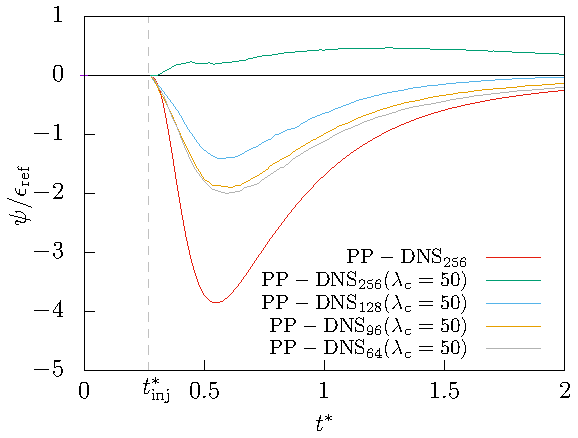
\includegraphics[width=\linewidth]{./Abbildungen/vergleich_coupling_time.pdf}
        \caption{Point-particle coupling rate $\Psi_\mathrm{pp}$ with constant $\lambda_\mathrm{c}$ for various resolutions. A relation of resolution and accuracy can be observed.}
        \label{vergleich_coupling_time_256}
    \end{minipage}
\end{figure}
\newline
The computational savings of this method may be present, their effect is not as prevalent as it needs to be to compensate the inaccurate results.
\pagebreak
\section{Conclusion and outlook}
In this work, two sets of simulations were carried out to evaluate a method for lowering computational effort. 
\newline
The results presented in this work show that for a sufficiently exact simulation particle clustering has to be treated with caution. Depending on the application maybe small numbers of clustered particles could be used, but the savings in computing time would not compensate the loss in accuracy. This is the case in particular high numbers of clustered particles at which the results get highly inaccurate. Maybe investigations on smaller numbers of clustered particles could follow, the space between 2 and 10 could be closed by simulations in the future to determine the real border for inaccurate results. 
\newline
Further investigation is needed regarding the second set of simulation (Fig. \ref{kineticEnergy_numberofparticles}), in which the goal was to find out which number of particles is necessary to get accurate results for the turbulent kinetic energy of the particles. The deviation of the averaged kinetic energy of the particles and the fluid should be zero. This difference converges to zero with high numbers of particles. The distribution of the experiment`s outcomes should match the well-known normal distribution, which leads to analyzing the standard deviation. Concluding, further simulations should be carried out until a sufficient standard deviation can be computed, from which an assumption about the accuracy of the initialization could be made.
\newline
%\subsection*{Acknowledgements}
%This work was supervised by Konstantin Fr\"ohlich, we would like to express our gratitude. Thank you for the chance of learning about turbulent flows and simulations, the advice and the deep insights in scientific work. We also appreciate the chance of writing this work at the Institute of Aerodynamics of the RWTH Aachen University.
\pagebreak
\section{References}
\nocite{*} %erm�glicht, dass auch Literatur, welche nicht zitiert wurde in der Bibliography auftaucht
\bibliography{Projektarbeit} %ruft die Bibliography-Datei auf
\bibliographystyle{plain} %setzt den Zitierstil
\pagebreak
\section{Appendix A}
\subsection*{Creating of pictures showing tubular structures}
The pictures used in to point out the differences between DNS and LES were generated using ParaView, an open-source-software developed by a joint-venture of Kitware and the Los Alamos National Laboratory. More information about the software can be found at www.paraview.org. To show the tubular structures in a turbulent flow, two filters were used: One was the AIALambda2Criterion1-Filter and the other one was the ISOVolume1-Filter. These filters were then set to visualize the velocity of the flow colored by magnitude. To diversify the different velocity-magnitudes, a rainbow-colorscheme was used. 
\end{document}
